\subsection{Enjeux}
\JulianSpeak
\begin{frame}{Enjeux}
\begin{itemize}
	\item Confirmer la position
	\begin{itemize}
		\item Améliorer son taux d'utilisation
		\item Étendre sa visibilité
		\item Faire de \bsc{Correlyce} une référence
	\end{itemize}
	\vfill
	\pause
	\item Logiciel libre
		\begin{itemize}
			\item Conserver la licence GPL
			\item S'inscrire dans la stratégie de région PACA
		\end{itemize}
			\vfill
	\pause			
	\item Expérience en agilité
\end{itemize}
\end{frame}
\subsection{Méthodologies et démarches}
\begin{frame}{Méthodologies et démarches}
	\begin{itemize}
		\item Une approche agile adaptée : KANBAN
		\item Allier la flexibilité de l'agilité et la maîtrise du risque
	\end{itemize}
	\begin{figure}[H]
		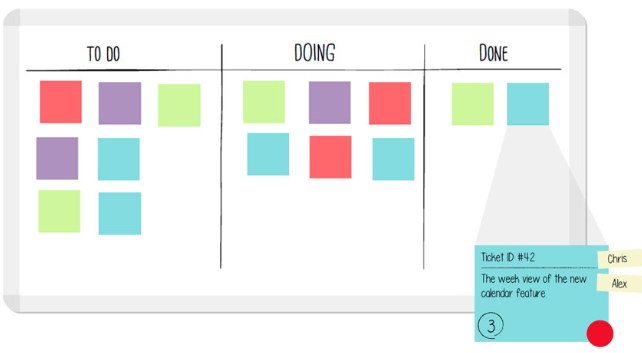
\includegraphics[width=8cm]{kanban.png}
		\caption{Fonctionnement du Board}
	\end{figure}
\end{frame}
\SteveSpeak
\subsection{Organisation de l'équipe}
\begin{frame}{Organisation de l'équipe}
		\begin{figure}[H]
			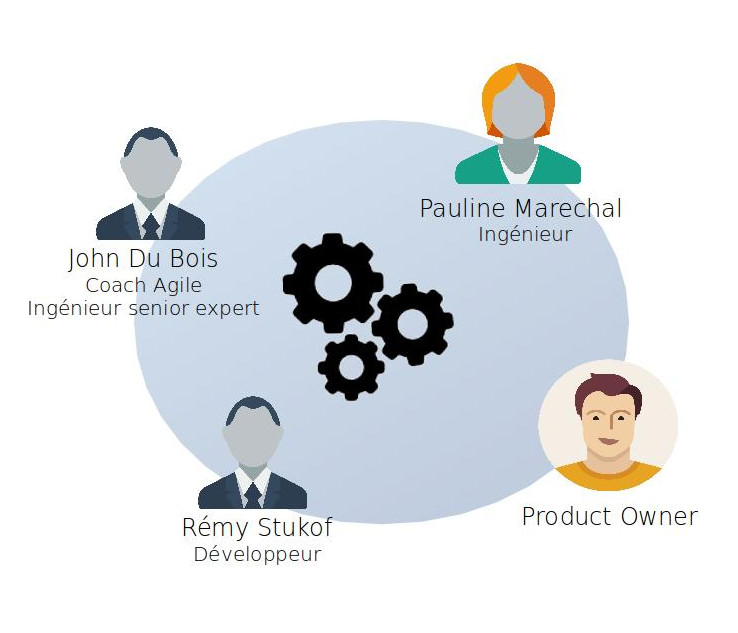
\includegraphics[width=8cm]{team.jpg}
			\caption{Organisation de l'équipe}
		\end{figure}
\end{frame}
\subsection{Moyens techniques}
\begin{frame}{Moyens techniques}
	\begin{itemize}
		\item Git et Github
		\item Travis CI
		\item Java (JUnit, CHeckStyle, PMD, Emma)
		\item SonarQube
		\item Heroku
		\item Zimbra
		\item Eclipse
	\end{itemize}
\end{frame}